\documentclass[twoside]{article}
\usepackage{mdframed}
\usepackage[hmarginratio=1:1,top=32mm,columnsep=20pt]{geometry} % Document margins
\usepackage{multicol} % Used for the two-column layout of the document
\usepackage[hang, small,labelfont=bf,up,textfont=it,up]{caption} % Custom captions under/above floats in tables or figures
\usepackage{booktabs} % Horizontal rules in tables
\usepackage{float} % Required for tables and figures in the multi-column environment - they need to be placed in specific locations with the [H] (e.g. \begin{table}[H])
\usepackage{hyperref} % For hyperlinks in the PDF
\usepackage{amsmath,amsthm,amssymb}
\usepackage{lettrine} % The lettrine is the first enlarged letter at the beginning of the text
\usepackage{paralist} % Used for the compactitem environment which makes bullet points with less space between them
\usepackage{tikz}
\usepackage{esint}
\usepackage{centernot}
\usepackage{lmodern}
\usetikzlibrary{3d}
\usetikzlibrary{patterns,calc,hobby}
\usetikzlibrary{decorations.pathreplacing}
\tikzset{
	partial ellipse/.style args={#1:#2:#3}{
		insert path={+ (#1:#3) arc (#1:#2:#3)}
	}
}
\usepackage{xcolor}

\usepackage{fancyhdr} % Headers and footers
\pagestyle{fancy} % All pages have headers and footers
\fancyhead{} % Blank out the default header
\fancyfoot{} % Blank out the default footer
\fancyhead[C]{Jimmy Yue $\bullet$ Statistics $\bullet$ Jimmy Yue} % Custom header text
\fancyfoot[RO,LE]{\thepage} % Custom footer text

\newmdenv[skipabove=7pt,
rightline=false,
leftline=true,
topline=false,
bottomline=false,
skipbelow=5pt,
linecolor=black,
innerleftmargin=5pt,
innerrightmargin=5pt,
innertopmargin=5pt,
leftmargin=0cm,
rightmargin=0cm,
linewidth=4pt,
innerbottommargin=5pt]{cBox}

\theoremstyle{definition}
\newtheorem*{solutionT}{Solution}

\newenvironment{solution}{\begin{cBox}\begin{solutionT}}{\hfill{\scriptsize\ensuremath{\square}}\end{solutionT}\end{cBox}}

%%%%%%%%%%%%%%%%%%%%%%%%%%%%%%%%%%%%%%%%%%%%%%%%%%%%%%%%%%%%%%%%%%%%%%%%%%%%%%%%%%%%%%%%%%%%
\newcommand{\vect}[1]{\vec{\pmb{#1}}}
\newcommand{\uvect}[1]{\hat{\mathbf{#1}}}
\newcommand{\leviciv}{\epsilon_{ijk}}

\newmdenv[skipabove=7pt,
rightline=false,
leftline=true,
topline=false,
bottomline=false,
skipbelow=5pt,
linecolor=black,
innerleftmargin=5pt,
innerrightmargin=5pt,
innertopmargin=5pt,
leftmargin=0cm,
rightmargin=0cm,
linewidth=4pt,
innerbottommargin=7,
backgroundcolor=light-gray]{dBox}



\theoremstyle{definition}
\newtheorem*{proof1}{Definition}

\newenvironment{ddef}{\begin{dBox}\begin{proof1}}{\hfill{\scriptsize}\end{proof1}\end{dBox}}
\newcommand{\pdif}[2]{\frac{\partial#1}{\partial#2}}
\definecolor{light-gray}{gray}{0.85}
%----------------------------------------------------------------------------------------
%-	TITLE SECTION
%----------------------------------------------------------------------------------------

\title{\vspace{-15mm}\fontsize{24pt}{10pt}\selectfont\textbf{Statistics - Week 3}} % Article title

\author{
\large
\textsc{Jimmy Tsz Ming Yue}\thanks{440159151}\\[2mm] % Your name
\normalsize University of Sydney \\ % Your institution
\normalsize \href{mailto:jyue6728@uni.sydney.edu.au}{jyue6728@uni.sydney.edu.au} % Your email address
\vspace{-5mm}
}
\date{}

%----------------------------------------------------------------------------------------

\usepackage{Sweave}
\begin{document}
\Sconcordance{concordance:week3.tex:week3.Rnw:%
1 331 1 1 2 1 0 1 2 1 0 4 1 4 0 1 2 6 1 1 4 3 0 4 1 3 0 1 3 1 0 4 1 4 0 %
1 5 3 0 4 1 3 0 1 3 1 0 4 1 4 0 1 2 1 4 3 0 4 1 3 0 1 3 1 0 4 1 4 0 1 5 %
3 0 4 1 3 0 1 3 1 0 4 1 4 0 1 2 3 1 1 2 1 0 1 1 5 0 5 1 9 0 1 1 9 0 1 1 %
10 0 1 3 1 0 3 1 4 0 1 2 5 1 1 2 1 0 3 1 3 0 1 3 1 0 2 1 6 0 1 4 6 1 1 %
2 1 0 1 2 1 0 4 1 4 0 1 2 5 1}

%\SweaveOpts{concordance=TRUE}

\maketitle % Insert title

\thispagestyle{fancy} % All pages have headers and footers
\hrule \smallskip

\noindent Semester 2 \quad Statistics \hspace{10.5
cm} 2018
\smallskip
\hrule
\smallskip
\tableofcontents

\section{Introduction to Density Estimation}
In this section of the unit we will introduce density estimation and smoothing methods. There are two types of methods classified as \emph{parametric} \emph{nonparametric}. Compared to \emph{parametric} methods \emph{nonparametric} methods lack of a formal statistical model. These methods are generally intended for description rather than formal inference. We learn such methods to describe the probability distribution of univariate random variable and multivariate random variables. 

\subsection{Usage of estimating a density function}
In exploratory data analysis, an estimate of the density function can be used: 
\begin{enumerate}
	\item to assess multimodality, skew, tail behaviour, etc
	\item in decision making, classifcation and summarising Bayesian posteriors.
	\item as a useful visulaisation tool. 
\end{enumerate}
In this section, the concern is the estimation of a density function $f$ using observations of random variables $x_1,  \dots x_n$ sampled independently from $f$. 

\section{Parametric density estimation}
The parametric approach to a density estimation assumes a parametric model, $x_1, \dots x_n \sim \text{i.i.d} f_\theta$ (where $\theta$ is a low-dimensional parameter vector). 

For example let us assume $x_i \sim N(m,s)$. We typically estimate parameters $\hat{\theta}$ using maximum likelihood. From this, density at $x$ can be estimated as $f(x|\hat{\theta})$. 

\begin{ddef}
	\textbf{Likelihood} The number that is the probability of some observed outcomes given a set of parameter values is regarded as the lieklihood of the set of parameter values given the observed outcomes. To put this in terms of probability densities; let us denote the probability density function assosciated with the outcomes $O$ as $f(O|\theta)$. Then we can estimate $\theta$ given observed outcomes $O$ by maximising the function:

	\begin{equation}
		L(\theta | O) = f(O | \theta)
	\end{equation}
\end{ddef}
Then let $f(x_1, x_2 \dots, x_n | \theta)$ be the probability of observing $x_1 \dots x_n$ given parameters $\theta$. (It should be a constant reminder that $\theta$ is the model and that $x_i$ are data. From this we have that:
	\begin{align*}
		f(x_1, \dots x_n | \theta) & = f(x_1| \theta)\cdot f(x_2| \theta)\cdot \dots \cdot  f(x_n| \theta) \\
	 	& = \prod_{i=1}^n f(x_i| \theta)
		\intertext{Then the likelihood function is defined as:}
		L(\theta | x_i) & = \prod_{i=1}^n f(x_i| \theta)
		 \intertext{as it is often easier to maximise log likelihoods we then have using log laws;}
		\text{ln} L(\theta | x_i) & = \sum_{i=1}^n \text{ln}f(x_i| \theta)
	\end{align*}
	\section{Non-Parametric Density Estimation}
	There are some dangers when using the parametric approaches that one should be careful of; When the assumed model $f_\theta$ is incorrect this approach can lead to serious inferential errors. We can use nonparametric approaches to density estimation, which: 
\begin{enumerate}
  \item Assume very little about the form of $f$.
  \item use local information to estimate $f$ at a point $x$. 
\end{enumerate}

An example of a nonparametric density estimator are Histograms which are a certain type of nonparametric density estimator, being piecewise constant density. Most mathematically packages support automatic histogram generation. 
\subsection{Histogram}
A histogram can be used as a simple visualisation of data. In a histogram, bins are first defined and then the number of data points within each bin is used to determine the height of the bar plot. With differing bin sizes histograms may look different. 


\section{Demonstrate histogram and parametric methods}

We can smooth out histograms using a smoother kernel, called a gaussian kernel density estimate. Each point contributes to a Gaussian curve to the total. This kernel is:

\begin{enumerate}
  \item A smooth density estimate derived from the data
  \item A powerful non-parametric model of the distribution of points. 
\end{enumerate}

\subsection{Kernel}


\begin{ddef}
  A kernel is a special type of probability density function which is symmetric. A kernel is a function and has the following properties:
  \begin{enumerate}
    \item Non-negative
    \item real-valued
    \item symmetric 
    \item Its definite integral over its support set must equal to $1$.
  \end{enumerate}
\end{ddef}

\subsubsection{Kernel Density Estimation}
Kernel Density Estimation is a non-parametric approach for estimating the probability density function(pdf) of a continuous random variable. It is non-parametric because it does not assume any underlying distribution for the variable. ($X$ does not need to be assumed to follow any specific distribution. ) At every point, a kernel function is created with the point at its centre. The kernel is symmetric around the point. We can estimate the probability density function is estimated by adding all of these kernel functions and dividing by the number of data to ensure that it satisfies the following:

\begin{enumerate}
  \item every possible value of the pdf is non-negative
  \item the definite integral of the pdf over its support set equals $1$ 
\end{enumerate}

The simple density estimator that weights all points within $h$ of $x$ equally is given by: 

\begin{equation}
\hat{f}(x) = \frac{1}{2hn} \sum^n_{i=1} 1_{\left\{x-Xi < h\right\}}
\end{equation}

A univariate kernel density estimator allows a more flexible weighting scheme, fitting 
\begin{equation}
\hat{f}(x) = \frac{1}{hn} \sum^n_{i=1} K \left( \frac{x - X_i}{h} \right)
\end{equation}

where $K$ is a kernel function and $h$ is a fixed number, called the bandwidth, window width or smoothing parameter. 

\subsubsection{Constructing a kernel density estimator}

\begin{enumerate}
  \item Choose a kernel; the common ones are normal (Gaussian), uniform (rectangular) and triangular. (Kernel functions are positive everywhere and symmetric at zero).
  \item At each point $X_p$ build the scaled kernel function 
  \begin{equation}
  \frac{1}{h}K \left[\frac{(x-X_i)}{h}\right]
  \end{equation}
  where $K$ is a kernel function and $h$ is a fixed number, called the bandwidth, window width or smoothing parameter. 
  \item Add the individual scaled kernel functions and divide by $n$;
  \begin{equation}
 \hat{f}(x) =  \frac{1}{nh}\sum^n_{i=1}K \left[\frac{(x-X_i)}{h}\right]
  \end{equation}
  this places a probability of $1/n$ to each $x_i$, which ensures the kernel density estimate integrates to $1$.
\end{enumerate}
Intuitvely we can think of distributions as the sum of many bumps.

\subsubsection{Choice of Kernels}

Kernel density estimation requires specifcation of two components; the kernel and the bandwith. 

The shape of the kernel has much influence on the results than does the bandwidth. We have the following examples;

\begin{enumerate}
\item Uniform:
\begin{equation}
k_0(u) = \frac{1}{2}(|u| \leq 1)
\end{equation}
\item Epanechnikov:
\begin{equation}
k_1(u) = \frac{3}{4}(1-u^2)(|u| \leq 1)
\end{equation}
\item Biweight:
\begin{equation}
k_2(u) = \frac{15}{16}(1-u^2)^2(|u| \leq 1)
\end{equation}
\item Triweight:
\begin{equation}
k_3(u) = \frac{35}{32}(1-u^2)^3(|u| \leq 1)
\end{equation}
\item Triweight:
\begin{equation}
k_\phi(u) = \frac{1}{\sqrt{2\pi}}\left( -\frac{u^2}{2}\right)
\end{equation}
\end{enumerate}

\section{Demonstrate Kernel Density Estimation}

The density estimator:
 \begin{equation}
 \hat{f}(x) =  \frac{1}{nh}\sum^n_{i=1}K \left[\frac{(x-X_i)}{h}\right]
  \end{equation}
  
  is a fixed-bandwidth kernel density estimator since $h$ is constant. The value chosen for the bandwith exerts a strong influence on the estimator $\hat{f}$. 
  \begin{enumerate}
  \item If $h$ is too small, the density estimator will tend to assign probability density too locally near observed data. 
  \item If $h$ is too large, the density estimator will spread probability density contributions too diffusely. 
  \end{enumerate}
  
  The bandwidth determines the trade-off between the bias and variance of estimator $\hat{f}$. 
  
  \begin{enumerate}
    \item A small bandwidth produces a density estimator with function indivative of high variability caused by under smoothing. 
    \item A large bandwidth causes important features of $f$ to be smoothed away, thereby causing bias. 
  \end{enumerate}
  
  The trade-off between the bias and the variane of an estimator is important in nearly all kinds of model selection. 
  \subsection{Integrated Squared Error}
  To evaluate $\hat{f}$ as an estimator of $f$ over the entire range of support, one could use the integrated squared error defined as:
  \begin{ddef}
  \textbf{ISE}
  \begin{equation}
  \text{ISE}(h) = \int^\infty_{-\infty}\left[\hat{f}(x) - f(x)\right]^2dx
  \end{equation}
  measuring the square of distances between $\hat{f}(x)$ to $f(x)$
  \end{ddef}
  To discuss the generic properties of an estimator, without reference to a particular observed sample, it is more sensible to average ISE(h) over all samples that might be oberved for which we can define:
  \begin{ddef}
	  \textbf{Mean Integrated Squared Error( MISE)} 
	  \begin{equation}
		  \text{MISE}(h) = E\left\{ \text{ISE}(h) \right\}
	  \end{equation}
  \end{ddef}
  \section{Cross-Validation }
  Cross-Validation, is a model validation for assessing how the results of a statistical analysis will generalise to an independent data set. We use this mainly when one wants to estimate how accurately a predicitve model will perform in practice. In a prediction problem, a model is usually given and we have a:
  \begin{enumerate}
  \item a dataset of known data on which training is run (training dataset)
  \item datset of unknown data against which the model is  tested. 
  \end{enumerate}
 
 \subsection{Goal of cross-validation}
 The goal of cross validation is to define a dataset to ``test'' the model in the training phase (validation dataset) in order to:
 \begin{enumerate}
	 \item limit problems like overfitting
	\item Give insight on how the model will generalise to an independent dataset.
 \end{enumerate}

 One round of cross-validation invovles:
 \begin{enumerate}
	 \item Partitiong a sample of data into complementary subsets,
	\item performing the analysis on one subset (called the training set) and 
	\item validating the analysis on the other subset (called the vaildation or the testing set)
 \end{enumerate}
 \subsection{Why use Cross-Validation} 

 Many bandwidth selection strategies begin by relating $h$ to
some measure of the quality of $\hat{f}$ as an estimator of $f$. The quality is quantified by some $Q(h)$, whose estimate $\hat{Q}(h)$, is optimised to find $h$. If $\hat{Q}(h)$ evaluates the quality of $\hat{f}$ based on how well it fits the observed data, this implies that observed data are being used twice:

\begin{enumerate}
\item Once to calculate $\hat{f}$ from the data and a 
\item second time to evaluate the quality of $\hat{f}$ as an estimator of $f$
\end{enumerate}

This double use prvodies an overoptimistif view of the quality of the estimator leading to overfitting. If we use cross-validation this problem is voided. 
\section{Spline Methods}
\subsection{Cubic Spline}
 A cubic spline is a piecewise cubic function that is everywhere twice differentiable.


\section{Tutorial}
The height.txt file (please download from week 3, Datasets Zip link and unzip the file)
contains heights of $100$ men and $100$ women measured in meters. There is another file
called newHeight.txt which contains additional heights of $10$ men and $10$ women.

\begin{enumerate}
\item Create an R markdown file, read in height.txt data and generate histogram to
summarise and visualise height variable.
\begin{solution}
We first read in the height file
\begin{Schunk}
\begin{Sinput}
> height <- read.delim("height.txt", header=TRUE)
> #head(height)
> name <- c("iD", "Height(m)")
> df <- data.frame(height)
> colnames(df) <- name
> heights <- as.numeric(df$"Height(m)")
> hist(heights)
\end{Sinput}
\end{Schunk}
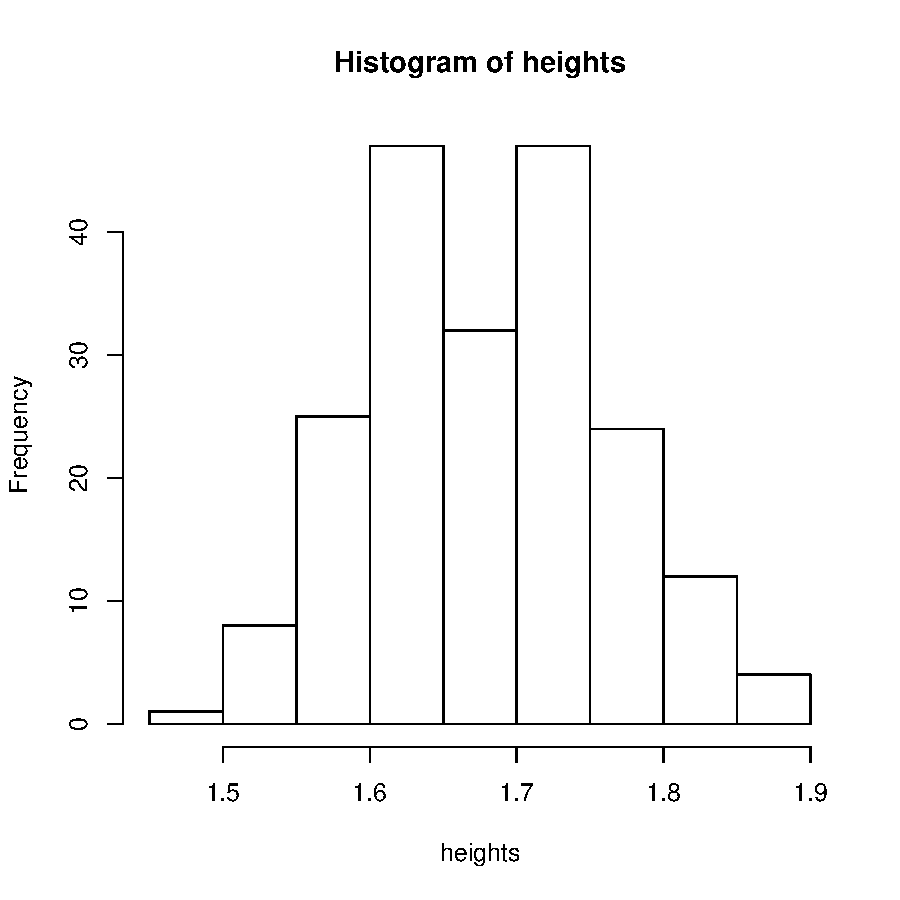
\includegraphics{week3-001}

\end{solution}
\item Apply kernel density estimation methods to estimate height density. Try different
kernel functions and bandwidths.

\begin{solution}
We use the density function in R:
\begin{Schunk}
\begin{Sinput}
> kernel = c("gaussian", "epanechnikov", "rectangular",
+                    "triangular", "biweight",
+                    "cosine", "optcosine")
> d1 <- density(heights, window = "gaussian", bw = 0.01)
> d2 <- density(heights, window = "gaussian", bw = 0.02)
> d3 <- density(heights, window = "gaussian", bw = 0.05)
> d4 <- density(heights, window = "gaussian", bw = 0.10)
\end{Sinput}
\end{Schunk}
\begin{Schunk}
\begin{Sinput}
> par(mfrow = c(2,2))
> plot(d1, main = "Heights")
> plot(d2, main = "Heights")
> plot(d3, main = "Heights")
> plot(d4, main = "Heights")
\end{Sinput}
\end{Schunk}
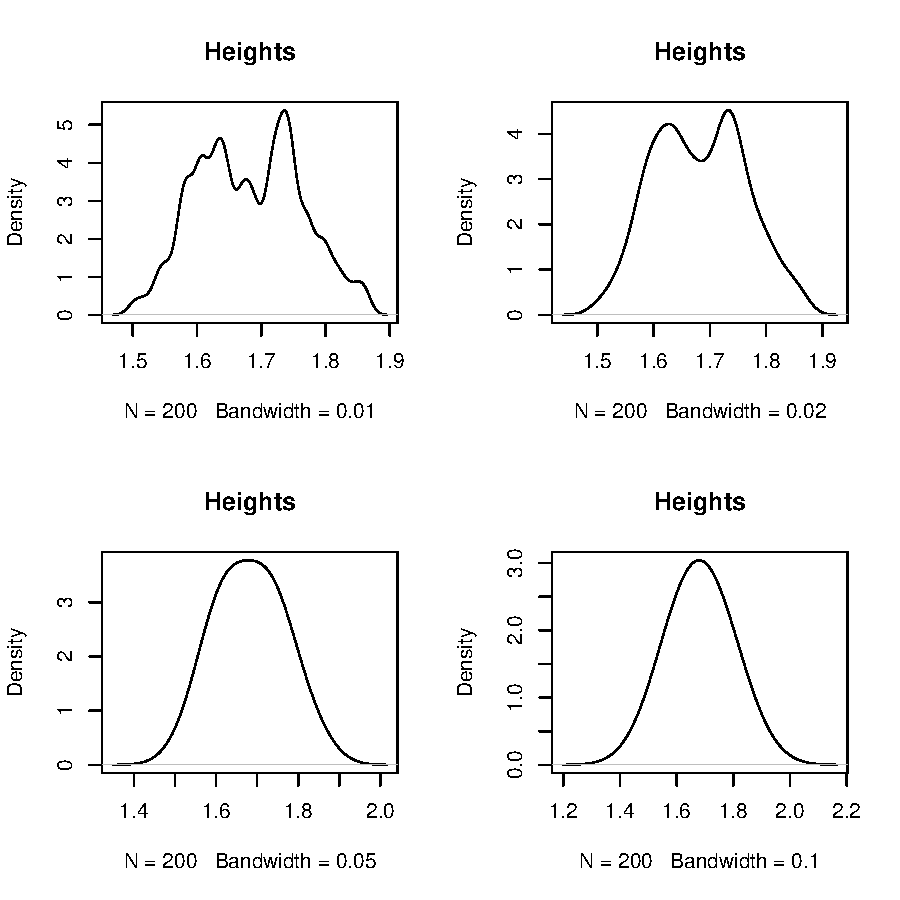
\includegraphics{week3-003}
\begin{Schunk}
\begin{Sinput}
> kernel = c("gaussian", "epanechnikov", "rectangular",
+                    "triangular", "biweight",
+                    "cosine", "optcosine")
> d1 <- density(heights, window = "epanechnikov", bw = 0.01)
> d2 <- density(heights, window = "epanechnikov", bw = 0.02)
> d3 <- density(heights, window = "epanechnikov", bw = 0.05)
> d4 <- density(heights, window = "epanechnikov", bw = 0.10)
\end{Sinput}
\end{Schunk}
\begin{Schunk}
\begin{Sinput}
> par(mfrow = c(2,2))
> plot(d1, main = "Heights")
> plot(d2, main = "Heights")
> plot(d3, main = "Heights")
> plot(d4, main = "Heights")
\end{Sinput}
\end{Schunk}
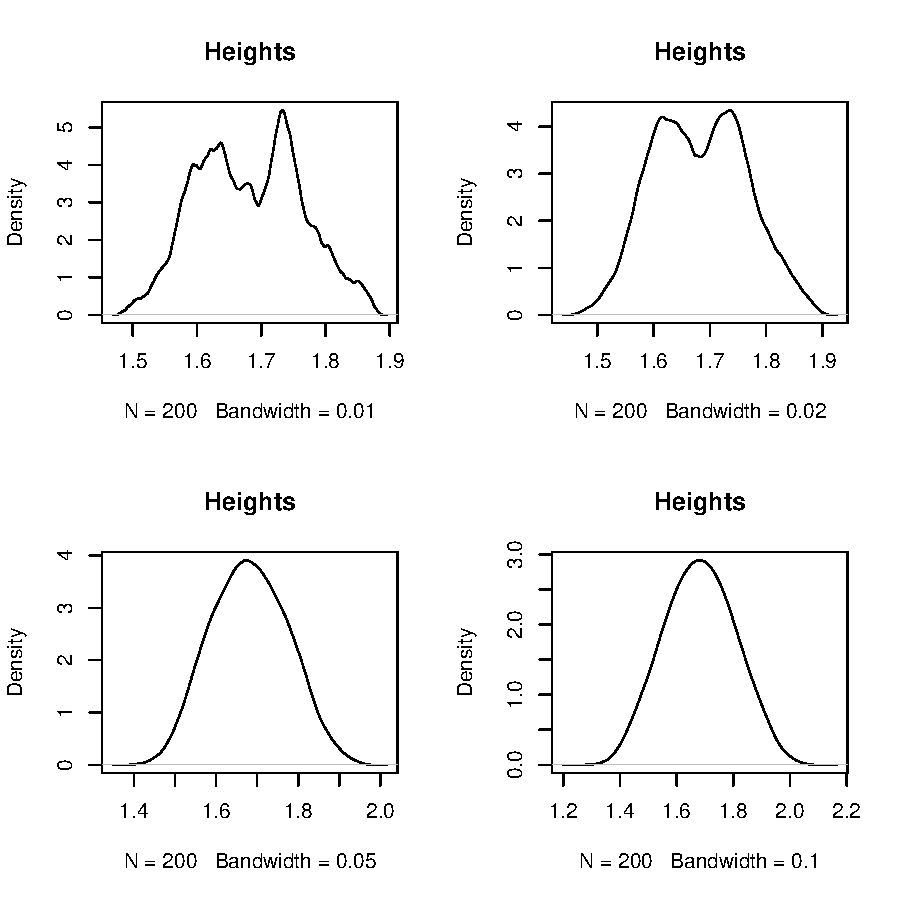
\includegraphics{week3-005}

\begin{Schunk}
\begin{Sinput}
> kernel = c("gaussian", "epanechnikov", "rectangular",
+                    "triangular", "biweight",
+                    "cosine", "optcosine")
> d1 <- density(heights, window = "rectangular", bw = 0.01)
> d2 <- density(heights, window = "rectangular", bw = 0.02)
> d3 <- density(heights, window = "rectangular", bw = 0.05)
> d4 <- density(heights, window = "rectangular", bw = 0.10)
\end{Sinput}
\end{Schunk}
\begin{Schunk}
\begin{Sinput}
> par(mfrow = c(2,2))
> plot(d1, main = "Heights")
> plot(d2, main = "Heights")
> plot(d3, main = "Heights")
> plot(d4, main = "Heights")
\end{Sinput}
\end{Schunk}
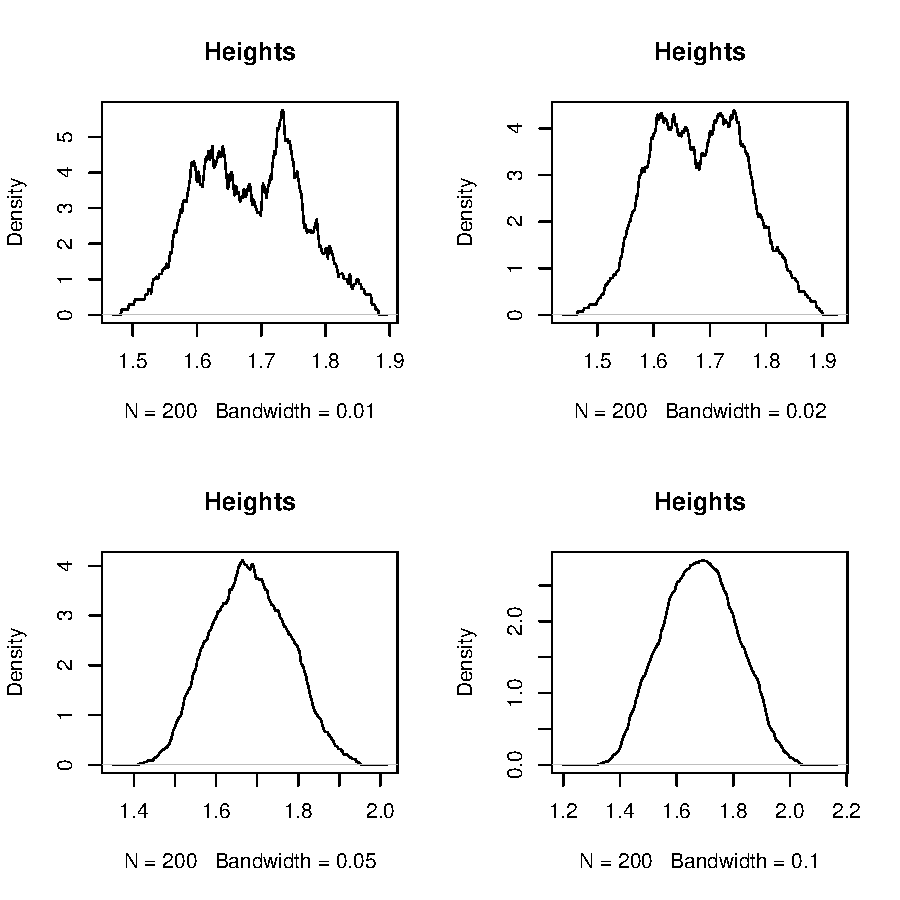
\includegraphics{week3-007}
\begin{Schunk}
\begin{Sinput}
> kernel = c("gaussian", "epanechnikov", "rectangular",
+                    "triangular", "biweight",
+                    "cosine", "optcosine")
> d1 <- density(heights, window = "biweight", bw = 0.01)
> d2 <- density(heights, window = "biweight", bw = 0.02)
> d3 <- density(heights, window = "biweight", bw = 0.05)
> d4 <- density(heights, window = "biweight", bw = 0.10)
\end{Sinput}
\end{Schunk}
\begin{Schunk}
\begin{Sinput}
> par(mfrow = c(2,2))
> plot(d1, main = "Heights")
> plot(d2, main = "Heights")
> plot(d3, main = "Heights")
> plot(d4, main = "Heights")
\end{Sinput}
\end{Schunk}
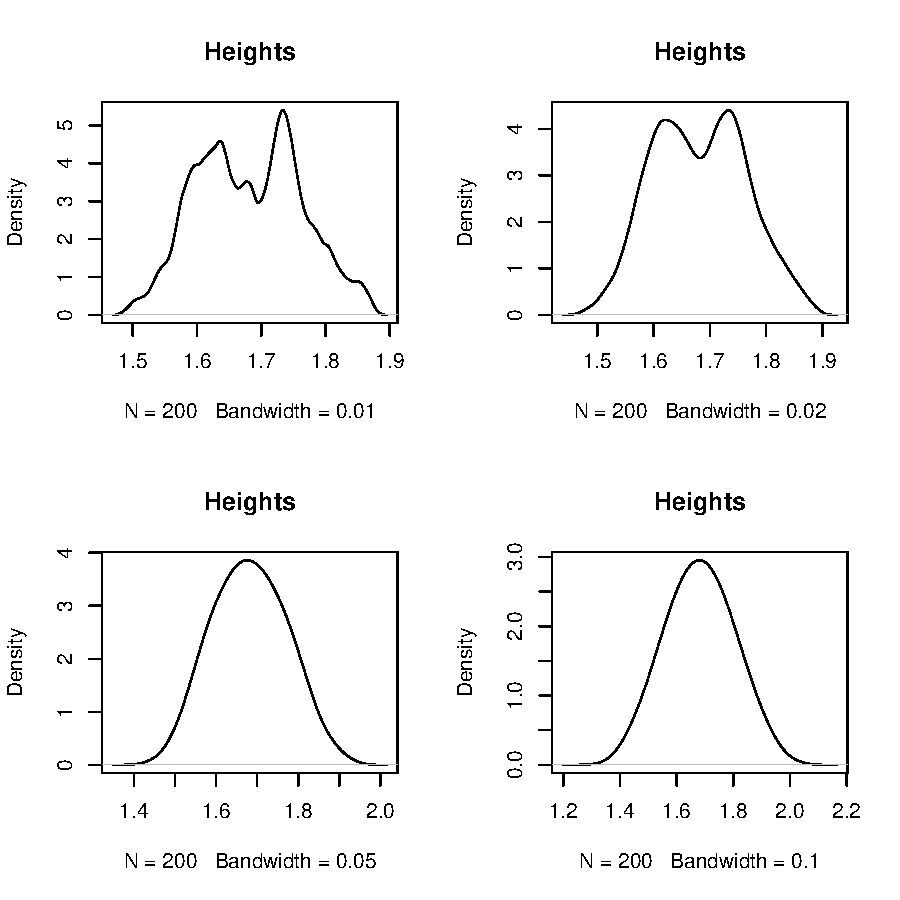
\includegraphics{week3-009}
\end{solution}
\item Use BCV methods to select for optimal bandwidth for each kernel of choice.
\begin{solution}
we use the bcv function in R:
\begin{Schunk}
\begin{Sinput}
> obw <- bw.bcv(heights)
> obw
\end{Sinput}
\begin{Soutput}
[1] 0.03196391
\end{Soutput}
\begin{Sinput}
> library(kedd)
> obw.gauss <- h.bcv(heights, kernel = "gaussian")
> obw.epan <- h.bcv(heights, kernel = "epanechnikov")
> obw.rect <- h.bcv(heights, kernel = "biweight")
> obw.rect
\end{Sinput}
\begin{Soutput}
Call:		Biased Cross-Validation 1

Derivative order = 0
Data: heights (200 obs.);	Kernel: biweight
Min BCV = 0.05189653;	Bandwidth 'h' = 0.107642
\end{Soutput}
\begin{Sinput}
> obw.epan
\end{Sinput}
\begin{Soutput}
Call:		Biased Cross-Validation 1

Derivative order = 0
Data: heights (200 obs.);	Kernel: epanechnikov
Min BCV = 0.2345472;	Bandwidth 'h' = 0.1418205
\end{Soutput}
\begin{Sinput}
> obw.gauss
\end{Sinput}
\begin{Soutput}
Call:		Biased Cross-Validation 1

Derivative order = 0
Data: heights (200 obs.);	Kernel: gaussian
Min BCV = 0.05893172;	Bandwidth 'h' = 0.04177944
\end{Soutput}
\end{Schunk}
\begin{Schunk}
\begin{Sinput}
> par(mfrow=c(2,2))
> plot(density(heights, window = "gaussian", bw =0.04))
> plot(density(heights, window = "epanechnikov", bw =0.14))
> plot(density(heights, window = "biweight", bw =0.10))
\end{Sinput}
\end{Schunk}
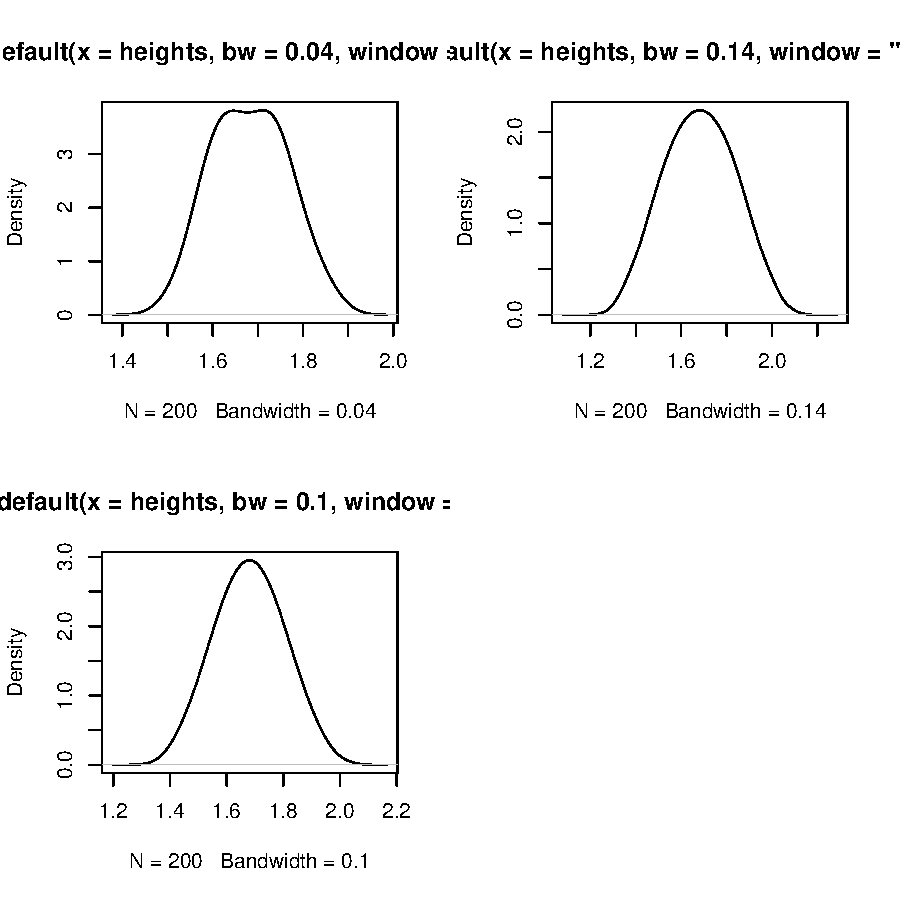
\includegraphics{week3-011}

\end{solution}
\item Apply cubic spline density estimation with different number of knots and compare
these results to those from using kernel functions.
\begin{solution}
We fist import the package and follow the given example
\begin{Schunk}
\begin{Sinput}
> library(polspline)
> fit1 <- logspline(heights)
> fit2 <- logspline(heights, nknots=5)
> fit3 <- logspline(heights, nknots=10)
\end{Sinput}
\end{Schunk}
\begin{Schunk}
\begin{Sinput}
> plot(fit1)
> plot(fit2, add=T,lty=2)
> plot(fit3, add=T,lty=3)
> 
> 
\end{Sinput}
\end{Schunk}
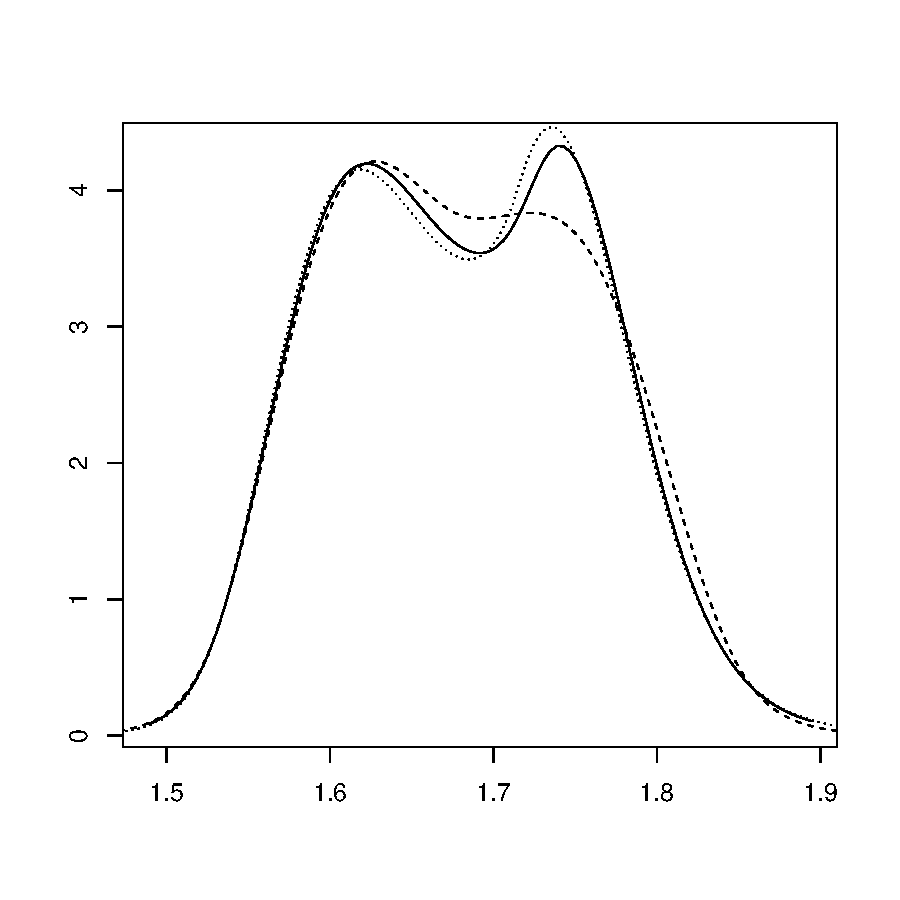
\includegraphics{week3-013}


\end{solution}
\item Read in newHight.txt data. Is it possible to classify each of these new samples in
newHight.txt dataset based on density estimation results from height.txt? Try to
perform such classification.
\begin{solution}
\begin{Schunk}
\begin{Sinput}
> newheight <- read.delim("newHeight.txt", header=TRUE)
> #head(height)
> name <- c("iD", "Height(m)")
> df <- data.frame(newheight)
> colnames(df) <- name
> newheights <- as.numeric(df$"Height(m)")
> hist(newheights)
\end{Sinput}
\end{Schunk}
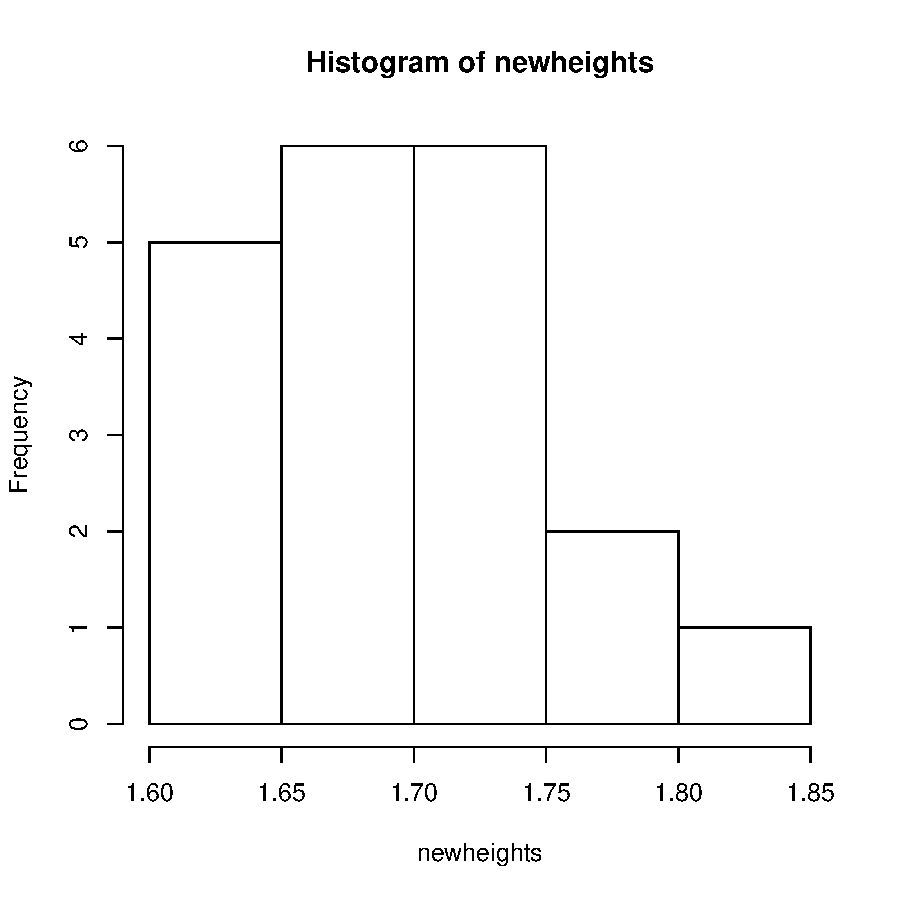
\includegraphics{week3-014}
We may make the estimation that the newheights may be drawn from the original distribution. However more validation on this is necessary 
\end{solution} 
\end{enumerate}


\end{document}
